\documentclass[11pt]{article}

\usepackage{amsmath, amssymb, amsthm}
\usepackage{tikz}

\theoremstyle{plain}
\newtheorem{thm}{Theorem}[section]
\newtheorem*{thm*}{Theorem}
\newtheorem{prop}[thm]{Proposition}
\newtheorem{lem}[thm]{Lemma}
\newtheorem*{lem*}{Lemma}
\newtheorem{dfn}[thm]{Definition}
\newtheorem{cor}[thm]{Corollary}
\newtheorem{claim}[thm]{Claim}
\newtheorem{conj}[thm]{Conjecture}
\newtheorem{ques}[thm]{Question}
\newtheorem*{rem}{Remark}


\oddsidemargin  0pt
\evensidemargin 0pt
\marginparwidth 40pt
\marginparsep 10pt
\topmargin 0pt
\headsep 10pt
\textheight 8.2in
\textwidth 6.4in
\renewcommand{\baselinestretch}{1.1}

\newcommand{\codeg}{\text{codeg}}
\newcommand{\BBE}{\mathbb{E}}
\newcommand{\BFP}{\mathbf{P}}
\usepackage{amsmath}
\usepackage{amsthm}
\usepackage{amssymb}
\usepackage{mathtools}
\usepackage{hyperref}
\usepackage{url}





\usepackage{graphicx}
\usepackage{caption}
\usepackage{subcaption}

\def\eQb#1\eQe{\begin{eqnarray*}#1\end{eqnarray*}}
\def\eQnb#1\eQne{\begin{eqnarray}#1\end{eqnarray}}
\providecommand{\e}[1]{\ensuremath{\times 10^{#1}}}
\providecommand{\pb}[0]{\pagebreak}
\DeclarePairedDelimiter\ceil{\lceil}{\rceil}
\DeclarePairedDelimiter\floor{\lfloor}{\rfloor}

\newcommand{\E}{\mathrm{E}}
\newcommand{\Var}{\mathrm{Var}}
\newcommand{\Cov}{\mathrm{Cov}}

\def\Qb#1\Qe{\begin{question}#1\end{question}}
\def\Sb#1\Se{\begin{solution}#1\end{solution}}


\newtheoremstyle{quest}{\topsep}{\topsep}{}{}{\bfseries}{}{ }{\thmname{#1}\thmnote{ #3}.}
\theoremstyle{quest}
\newtheorem*{definition}{Definition}
\newtheorem*{theorem}{Theorem}
\newtheorem*{lemma}{Lemma}
\newtheorem*{question}{Question}
\newtheorem*{preposition}{Preposition}
\newtheorem*{exercise}{Exercise}
\newtheorem*{challengeproblem}{Challenge Problem}
\newtheorem*{solution}{Solution}
\newtheorem*{remark}{Remark}
\usepackage{verbatimbox}
\usepackage{listings}
\usepackage{mathrsfs}
\date{}
\title{\vspace{-0.7cm}
Atiyah Commutative Algebra: Problems}

\author{
Youngduck Choi 
\thanks{Department of Mathematics, Courant Institute of Mathematical Sciences, 
yc1104@nyu.edu; If you find an error and want to share with me, 
you can reach me via email.
}}

\begin{document}

\maketitle

\begin{abstract}
This work contains solutions to some
exercises from Atiyah's Commutative Algebra
text.
\end{abstract}


\section{Chapter 2: Modules} \label{sec:Modules}

\begin{question}[2.1]
\hfill
\begin{figure}[h!]
  \centering
    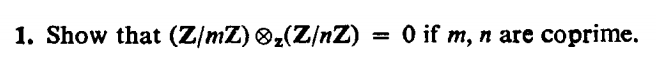
\includegraphics[width=0.7\textwidth]{d-2-1.png}
\end{figure}
\end{question}
\begin{solution} \hfill \\
As $m,n$ are coprime, by Bezout, there exists $a,b \in \mathbb{Z}$ such that
\eQb
am + bn = 1.
\eQe
Therefore, 
\eQb
x \otimes y &=& am(x \otimes y) + bn(x \otimes y) = a (mx \otimes y) + 
b(x \otimes ny) = a(0 \otimes y ) + b(x \otimes 0) = 0 
\eQe
for any $x \otimes y \in \mathbb{Z}/n\mathbb{Z} 
\otimes_{\mathbb{Z}} \mathbb{Z}/m\mathbb{Z}$. 
\hfill $\qed$

\end{solution}

\bigskip

\begin{question}[2.4]
\hfill
\begin{figure}[h!]
  \centering
    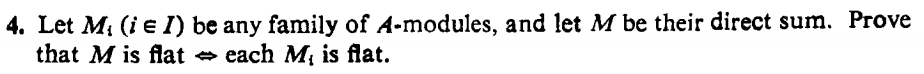
\includegraphics[width=0.7\textwidth]{d-2-4.png}
\end{figure}
\end{question}
\begin{solution} \hfill \\
Let $M = \bigoplus_{i \in I} M_i$. Then, $M$ is exact iff for any exact sequence
of $A-$modules
\eQb
0 \to N' \to N \to N'' \to 0 
\eQe 
the tensored sequence 
\eQb
0 \to N' \otimes M \to N \otimes M \to N'' \otimes M \to 0 
\eQe 
is exact. Observe that the above tensored sequence can be written as
\eQb
0 \to \bigoplus_{i \in I} N' \otimes M_i \to 
\bigoplus_{i \in I} N \otimes M_i \to
\bigoplus_{i \in I} N'' \otimes M_i \to 0. 
\eQe
Hence $M$ is exact iff for any $i \in I$ and for any exact sequence of $A-$modules
\eQb
0 \to N' \to N \to N'' \to 0 
\eQe
the tensored sequence
\eQb
0 \to N' \otimes M_i  \to N \otimes M_i \to N'' \otimes M_i \to 0, 
\eQe
but the later is equivalent to $M_i$ being flat for all $i \in I$, so we are done.
\hfill $\qed$

\end{solution}

\bigskip

\begin{question}[2.5]
\hfill
\begin{figure}[h!]
  \centering
    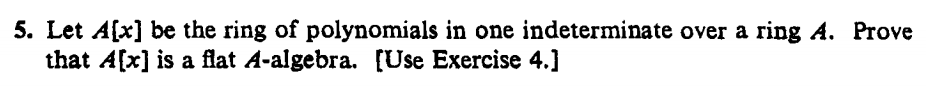
\includegraphics[width=0.7\textwidth]{d-2-5.png}
\end{figure}
\end{question}
\begin{solution} \hfill \\

\end{solution}

\section{Chapter 6: Chain Conditions} \label{sec:CC}

\begin{question}[6.2]
\hfill
\begin{figure}[h!]
  \centering
    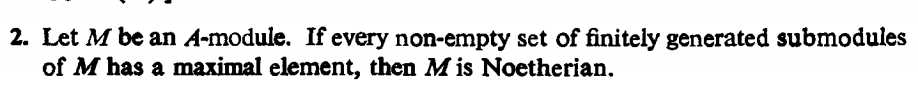
\includegraphics[width=0.7\textwidth]{d-6-2.png}
\end{figure}
\end{question}
\begin{solution} \hfill \\
Suppose $M$ is not Noetherian. Then, there exists a non finitely-generated submodule
$N$ of $M$. Choose $x_1$ from $N$. Then, since $N$ is non finitely-generated,
$N - \{ x_1 \} \neq \emptyset$, so we can choose $x_2 \neq x_1$ from $N$. Repeat
this process inductively, then we have a nonempty set of finitely generated
submodules of $M$ 
\eQb
\{ (x_1), (x_1, x_2), (x_1, x_2, x_3) ... \}
\eQe
such that it does not have a maximal element. Therefore, by contradiction,
we have that $M$ must be Noetherian. \hfill $\qed$  

\end{solution}

\bigskip

\section{Chapter 3: Rings and Modules of Fractions} \label{sec:RMF}
\begin{question}[3.1]
\hfill
\begin{figure}[h!]
  \centering
    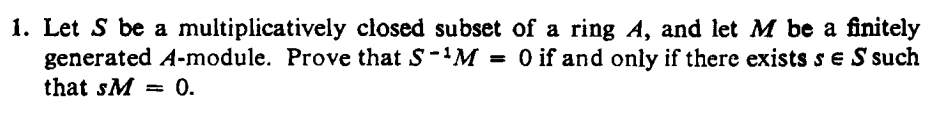
\includegraphics[width=0.7\textwidth]{d-3-1.png}
\end{figure}
\end{question}
\begin{solution} \hfill \\
Suppose there exists $s_0 \in S$ such that $s_0 M = 0$. Then, for any 
$(a,s), (b,t) \in A \times S$,  
\eQb
(at - bs) s_0 = 0
\eQe
so $(a,s) \sim (b,t)$, and hence $S = 0$. 
Conversely, suppose $S^{-1}M = 0$. As $M$ is finitely generated,
there exists $\{x_1 , ..., x_m\}$ for some $m$ that generates $M$. As $S^{-1}M = 0$,
we can choose $\{s_1, ..., s_m\}$ such that
\eQb
s_i x_i = 0
\eQe 
for all $1 \leq i \leq m$. Consider $s^* = s_1...s_m$. Then,
\eQb
s^* x &=& s_1...s_m x = s_1 ... s_m (\sum_{i=1}^{m} a_i x_i ) \\
&=& \sum_{i=1}^{m} s_1 ... s_m a_i x_i =  0  
\eQe 
for some $a_1,...a_m \in A$, for all $x \in M$. Therefore, $s^*M = 0$.
\hfill $\qed$

\end{solution}

\bigskip

\begin{question}[3.2]
\hfill
\begin{figure}[h!]
  \centering
    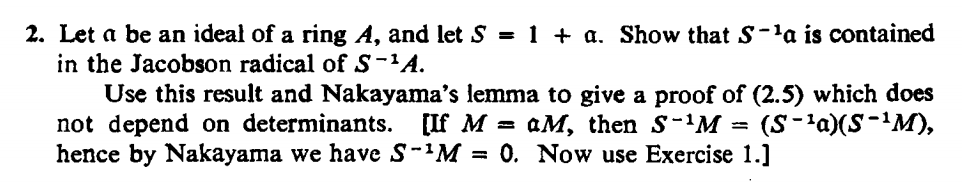
\includegraphics[width=0.7\textwidth]{d-3-2.png}
\end{figure}
\end{question}
\begin{solution} \hfill \\
If $1+a, 1+a' \in 1+ \textbf{a}$, then
\eQb
(1+a)(1+a') &=& 1 a + a' + aa' \in 1 + \textbf{a}. 
\eQe 
Therfore $1+\textbf{a}$ is a multiplicatively closed set in $A$. Now,
for any $\in 1 + \textbf{a}$, 
\eQb
1 - 1
\eQe

\end{solution}

\bigskip

\begin{question}[3.12]
\hfill
\begin{figure}[h!]
  \centering
    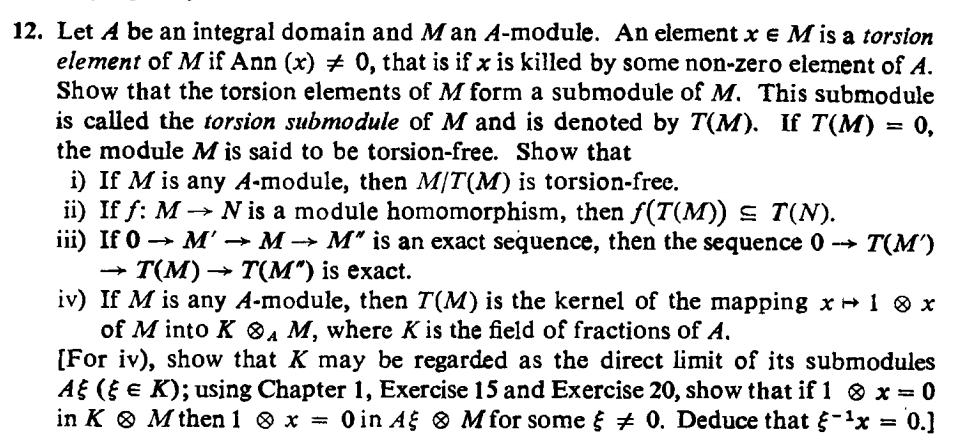
\includegraphics[width=0.7\textwidth]{d-3-12.png}
\end{figure}
\end{question}
\begin{solution} \hfill \\
If $1+a, 1+a' \in 1+ \textbf{a}$, then
\eQb
(1+a)(1+a') &=& 1 a + a' + aa' \in 1 + \textbf{a}. 
\eQe 
Therfore $1+\textbf{a}$ is a multiplicatively closed set in $A$. Now,
for any $\in 1 + \textbf{a}$, 
\eQb
1 - 1
\eQe
ddd
\end{solution}

\bigskip

\begin{question}[3.13]
\hfill
\begin{figure}[h!]
  \centering
    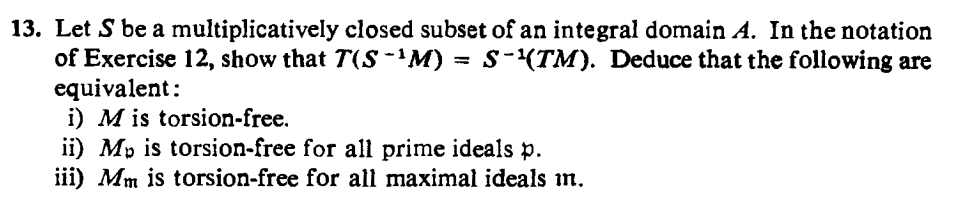
\includegraphics[width=0.7\textwidth]{d-3-13.png}
\end{figure}
\end{question}
\begin{solution} \hfill \\
\end{solution}



\end{document}
